%----------------------Pre-Amble-------------------------
\documentclass{MathNotes}
%----------------------Author Information-----------------
\title{Math-2417.001 Notes}
\author{Minh Nguyen}

%---------------------Document Begin-----------------------
% \usepackage{layout}
\begin{document}
% \begin{center}
%     \layout*
% \end{center}
\newpage
\maketitle
\pagenumbering{roman}
\tableofcontents
\newpage
\section*{Author's Notes}
This is my very first project that I wrote in \LaTeX, but I hope you enjoy
the notes that I poured my blood, sweat, and tears into \emoji{sob} 
\br
These notes are based off of the textbook \textit{Calculus 11e} by 
\textit{Ron Larson} and \textit{Bruce Edwards}, as well as the lectures of 
professor \textit{Carlos Arreche}.
\br
If you have any complaints, or suggestions regarding these notes, please
email me at \href{mailto:minh.nguyen7@utdallas.edu}{mdn220004@utdallas.edu}
\newpage
\pagenumbering{arabic}

\section{Limits}\label{sec:1}
\subsection{Introduction to Calculus --- "Mathematics of Change"}

You can use calculus to study static objects by pretending they're changing
\\

\begin{example}{}
    A circle has area $\pi r^2$, but you can use the radius $r$ to calculate
    the area of other polygons, such as a square, triangle, pentagon, etc\dots
    \\

    In other words, the \textit{limit} of the areas inscribed polygons in a circle
    is $\pi r^2$
\end{example}

\subsection{Finding Limits Graphically \& Numerically}

\begin{multicols}{2}[]
\begin{theorem}{Informal Definition of Limit}
    \[\lim_{x\to c}f(x)=L\] 
    As $x$ gets closer to $c$, the value of $f(x)$ becomes $L$
\end{theorem}


Limits also depend on what direction\footnote{If the limits from the left and
right don't match, then the limit \textit{doesn't exist}} you're coming from:
\begin{tabular}{ |l|c| }
    \hline
    Meaning & Math Expression\\
    \hline
    \hline
    From the right & $\lim_{x\to c^+}f(x)$ \\
    \hline
    From the left & $\lim_{x\to c^-}f(x)$ \\
    \hline
\end{tabular}
\end{multicols}

\begin{example}{Estimating Graphically and Numerically}\label{ex:1.2}
    Consider the function $f(x)=\frac{x^3-1}{x-1}$:
    \begin{center}
        \begin{tikzpicture}
            \begin{axis}[
                    axis lines        = box,
                    xmin              = 0,
                    xmax              = 2,
                    ymin              = 0,
                    ymax              = 8,
                    xlabel            = $x$,
                    ylabel            = $f(x)$,
                    variable          = t,
                    trig format plots = rad,
                ]

                \addplot [
                    domain=0:2,
                    smooth,
                    color=blue,
                ]
                {(x^3-1)/(x-1)};
                \addlegendentry{$f(x)=\frac{x^3-1}{x-1}$}

                \addplot [
                    color=blue,
                    mark=o
                ]
                coordinates {(1,3)};
            \end{axis}
        \end{tikzpicture}

        \begin{tabular}{ |c||c|c|c|c|c|c|c| }
            \hline
            x    & 0.9 & 0.99 & 0.999 & 1 & 1.001 & 1.01 & 1.1\\
            \hline
            f(x) & 2.71 & 2.97 & 2.997 &DNE& 3.003 & 3.03 & 3.31 \\
            \hline
        \end{tabular}
    \end{center}

    Notice how in both the \textbf{table and graph}, $f(x)$ looks like it's
    approaching $f(x)=3$ when $x=1$
\end{example}

\subsubsection{When Limits Fail to Exist}
\begin{note}{Limits Don't Exist When}
    \begin{itemize}
        \item $\lim_{x\to c^-}f(x)\neq \lim_{x\to c^+}f(x)$
        \item $f(x)$ is a violently oscillating function
    \end{itemize}
\end{note}

\subsubsection{A Formal Definition}

\begin{multicols}{2}[
        Basically...
    ]
    \begin{theorem}{Limits via. $\varepsilon - \delta$}
        The statement $\lim_{x\to c}f(x)=L$ means that for each $\varepsilon > 0$ there 
        exists $ \delta>0 $ such that if $0<\lvert x-c \rvert < \delta$ then
        $\lvert f(x)-L \rvert < \varepsilon$
    \end{theorem}

    \begin{center}
        \begin{tikzpicture}
            \begin{axis}[
                    scale only axis,
                    width  = 5cm,
                    xmin   = 0,
                    xmax   = 0.85,
                    ymin   = 0,
                    ymax   = 1,
                    xtick  = \empty,
                    ytick  = \empty,
                    xlabel = \empty,
                    ylabel = \empty,
                    clip   = false,
                    smooth,
                ]

                \addplot[
                    domain=0:0.85, 
                    samples=100, 
                    color=red,
                ]{sqrt(x)};

                % add open dot for removable discontinuity
                \addplot [
                    color=blue,
                    mark=o
                ] coordinates {(0.4225,0.65)};

                % Epsilon-delta lines
                \draw [dashed, blue] (0, 0.75) -- (0.5625, 0.75);
                \draw [dashed, blue] (0, 0.65) -- (0.4225, 0.65);
                \draw [dashed, blue] (0, 0.55) -- (0.3025, 0.55);
                \draw [dashed, blue] (0.5625, 0) -- (0.5625, 0.75);
                \draw [dashed, blue] (0.4225, 0) -- (0.4225, 0.65);
                \draw [dashed, blue] (0.3025, 0) -- (0.3025, 0.55);

                % Labels
                \node[below] at (0.5625, 0) {c + \delta};
                \node[below] at (0.4225, 0) {c};
                \node[below] at (0.3025, 0) {c - \delta};
                \node[left] at (0, 0.75) {L + \varepsilon};
                \node[left] at (0, 0.65) {L};
                \node[left] at (0, 0.55) {L - \varepsilon};
                \node[right] at (0.4225, 0.65){(c, L)};

            \end{axis}
        \end{tikzpicture}
    \end{center}
\end{multicols}
Refer back to finding limits numerically (example \ref{ex:1.2}):
\begin{itemize}
    \item $\pm\varepsilon$ would be the values on the row $f(x)$
    \item $\pm\delta$ would be the values on the row $x$
\end{itemize}


\begin{example}{Proving Limits via. $\varepsilon-\delta$ Definition}
    Consider $f(x)=10x-6$, prove that $\lim_{x\to 3}f(x)=24$ using the 
    $\epsilon-\delta$ definition:
    \br
    The first thing we would have to do is to find $\delta$:
    \begin{align*}
        \lvert (10x-6)-(24) \rvert &<\varepsilon  \\
        \lvert 10x-30 \rvert &<\varepsilon \\
        10\lvert x-3 \rvert &<\varepsilon \\
        \lvert x-3 \rvert &<\frac{\varepsilon}{10}
    \end{align*}
    \begin{align*}
        0 < \lvert x - (3)\rvert &< \delta
    \end{align*}

    Notice how $\delta=\frac{\epsilon}{10}$. This guarantees that
    $\lvert f(x)-L \rvert < \epsilon$ whenever $0<\lvert x-c \rvert<\delta$
\end{example}

\newpage
\subsection{Evaluating Limits Analytically}

\subsubsection{Properties of Limits}

\marginpar{$\mathbb{R}=$all real numbers\\$\mathbb{N}=$all natural numbers}
\begin{multicols}{2}[]
    \begin{theorem}{Basic Limit Properties}
        Let $\{b, c\}=\mathbb{R}$, $n=\mathbb{N}$:

        \begin{enumerate}
            \item $\lim_{x\to c}x=c$ 
            \item $\lim_{x\to c}b=b$ 
            \item $\lim_{x\to c}x^n=c^n$
        \end{enumerate}
    \end{theorem}

    \begin{example}{Evaluating Basic Limits}
        \begin{center}
            \begin{align*}
                \lim_{x\to 2}5&=5 \\  
                \lim_{x\to 4}x&=4 \\
                \lim_{x\to 5}x^2&=25
            \end{align*}
        \end{center}
    \end{example}
\end{multicols}

\marginpar{$f(g(x))$ may also be written as $f\circ g$ }
\begin{theorem}{Limit Properties}
    Let $\{b, c\}=\mathbb{R}$, $n=\mathbb{N}$, and $f$ and $g$ are functions
    with limits:
    \begin{displaymath}
        \lim_{x\to c}f(x)=L\hspace{2ex}\text{and}\hspace{2ex}\lim_{x\to c}g(x)=K
    \end{displaymath}

    \begin{enumerate}
        \item $\lim_{x\to c}\l[ b\cdot f(x) \r]=b\cdot L$
        \item $\lim_{x\to c}\l[ b\pm f(x) \r]=b\pm L$
        \item $\lim_{x\to c}\l[ f(x)\cdot g(x) \r]=L\cdot K$
        \item $\lim_{x\to c}\frac{f(x)}{g(x)}=\frac{L}{K}, K\neq 0$
        \item $\lim_{x\to c}\l[ f(x)\r] ^n=L^n$
        \item $\lim_{x\to c}\sqrt[n]x=\sqrt[n]{c}$
        \item $\lim_{x\to c}f\bigl(g(x)\bigr)=f\bigl(\lim_{x\to c}g(x)\bigr)=f(K)$
    \end{enumerate}
\end{theorem}

\begin{example}{Limit of Polynomial}
    Evaluate $\lim_{x\to 5}\lbrack 3x^3 + 4 \rbrack$:
    \br
    \begin{align*}
        \lim_{x\to 5}\l[ 3x^3+4 \r] &= \lim_{x\to 5} 3x^3 + \lim_{x\to 5}4\\
        &= 3 \cdot \lim_{x\to 5}x^3 + \lim_{x\to 5}4\\
        &= 3 \cdot (5)^3 + 4 \\
        &=379
    \end{align*}
\end{example}

\begin{theorem}{Limits of Polynomial/Rationals}
    Let $c=\mathbb{R}$ and $p$ be a polynomial function:
    \begin{displaymath}
        \lim_{x\to c}p(x)=p(c)
    \end{displaymath}

    Let $r$ be a rational function $r(x)=\frac{p(x)}{q(x)}$ and $c=\mathbb{R}$
    such that $q(c)\neq 0$:

    \begin{displaymath}
        \lim_{x\to c}r(x)=r(c)=\frac{p(r)}{q(r)}
    \end{displaymath}
\end{theorem}

\newpage
\subsubsection{Squeeze Theorem}\label{sec:1.3.2}

\marginpar{
    Open/closed interval continuity will be discussed later in section
    \ref{sec:1.4.1}. 
}
\begin{multicols}{2}[]
    \begin{theorem}{The Squeeze Theorem}
        Suppose $h(x)\leq f(x) \leq g(x)$ for all $x$ in an open interval
        \textit{except} when $x=c$
        \br

        Also suppose that $\lim_{x\to c}h(x)=L=\lim_{x\to c}g(x)$ i.e. they share
        the same limit.
        \br

        This would mean that $\lim_{x\to c}f(x)=L$
    \end{theorem}

    \begin{theorem}{Trigonomic Limits}
        \begin{enumerate}
            \item $\lim_{x\to 0}\frac{\sin x}{x}$
            \item $\lim_{x\to 0}\frac{1 - \cos x}{x} = 1$
        \end{enumerate}
    \end{theorem}

    \begin{center}
        \begin{tikzpicture}
            \begin{axis}[
                    axis lines        = box,
                    xmin              = -5,
                    xmax              = 5,
                    ymin              = -5,
                    ymax              = 5,
                    xtick             = \empty,
                    ytick             = \empty,
                    xlabel            = \empty,
                    ylabel            = \empty,
                    trig format plots = rad,
                    width             = 15em,
                    title             = {Squeeze Theorem}
                ]

                \addplot [
                    smooth,
                    color=red,
                ]{x^2};
                \addplot [
                    smooth,
                    color=green,
                ]{-x^2};

                % add shading to regions

                \addplot [
                    draw=none,
                    pattern = north west lines,
                    pattern color=red,
                    smooth,
                ]{x^2};
                \addplot [
                    smooth,
                    draw=none,
                    pattern = north west lines,
                    pattern color=green,
                ]{-x^2};


                \addplot [
                    smooth,
                    color=blue,
                ]{x * sin(x)};

                \addplot [
                    color=black,
                    mark=*,
                ]coordinates{(0, 0)};

                \node[right] at (0, 0) {(c, L)};
            \end{axis}
        \end{tikzpicture}
    \end{center}
\end{multicols}

\subsection{Continuity}

\begin{definition}{Definition of Continuity}
    A function $f$ is continuous if:
    \begin{enumerate}
        \item $f(c)$ exists
        \item $\lim_{x\to c}f(x)$ exists
        \item $f(c)=\lim_{x\to c}f(c)$
    \end{enumerate}
\end{definition}

\marginpar{$\therefore$ means "therefore"}
\begin{example}{Determine Continuity}
    Determine if the function is continuous at $x=2$

    \begin{displaymath}
        f(x) = \begin{cases}
            \frac{x^2-x-2}{x-2} &\text{for } x\neq 2\\
            1 &\text{for } x=2
        \end{cases}
    \end{displaymath}
    \br

    We should probably start by plugging in $x=2$ for the case that
    $x\neq2$ to see if it equals the case where $x=2$:
    \begin{displaymath}
        \frac{x^2-x-2}{x-2}=\frac{(2)^2-(2)-2}{(2)-2}=\frac{0}{0}
    \end{displaymath}

    That's so \textit{uncool}. Let's factor it out and try again!
    \begin{align*}
        \frac{x^2-x-2}{x-2} = \frac{(x-2)(x+1)}{x-2} &= x+1\\
        &=(2)+1\\
        &=3
    \end{align*}

    Now, we compare both that with the case where $x=2$ to see if they
    are the same: $3\neq2$

    $\therefore f(x)$ is \textit{not continuous} at $x=2$!

\end{example}
\newpage

\begin{note}{Continuous Functions}
    The following functions are always continuous \textit{everywhere
    they're defined}:
    \begin{itemize}
        \item polynomial functions
        \item rational functions
        \item radical functions
        \item trigonomic functions
    \end{itemize}
\end{note}

\subsubsection{Open and Closed Intervals}\label{sec:1.4.1}
A function is continuous on an \textbf{open interval} $(a, b)$ if
$f(x)=c$ for each $c$ in $(a, b)$

A function is continuous on a \textbf{closed interval} $[a, b]$ if:
\begin{itemize}
    \item $f(x)$ is continuous on $(a, b)$
    \item $\lim_{x\to b^-}f(x)=f(b)$
    \item $\lim_{x\to a^+}f(x)=f(a)$
\end{itemize}

\begin{theorem}{Intermediate Value Theorem}
    If $f(x)$ is continuous on $[a, b], a\neq b$, and $k$ is any number
    between $f(a)$ and $f(b)$, then there exists a number $c$ in
    $[a, b]$ such that: $$f(c)=k$$
\end{theorem}

\subsubsection{Discontinuities}

\begin{multicols}{2}[
        There are two cases where discontinuities happen:
        \marginpar{Another example of removable discontinuity is in
        example \ref{ex:1.2}}
    ]{
        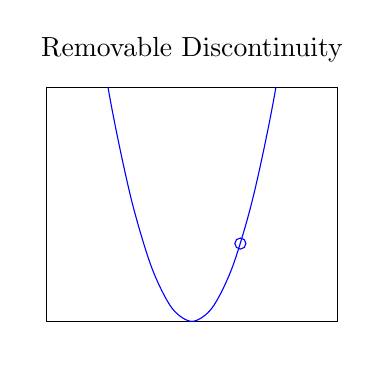
\begin{tikzpicture}
            \begin{axis}[
                    axis lines        = box,
                    xmin              = -3,
                    xmax              = 3,
                    ymin              = 0,
                    ymax              = 3,
                    xtick             = \empty,
                    ytick             = \empty,
                    xlabel            = \empty,
                    ylabel            = \empty,
                    trig format plots = rad,
                    width             = 15em,
                    title             = {Removable Discontinuity}
                ]

                \addplot [
                    smooth,
                    color=blue,
                ]{x^2};

                \addplot [
                    color=blue,
                    mark=o
                ]coordinates {(1,1)};
            \end{axis}
        \end{tikzpicture}
        \\
        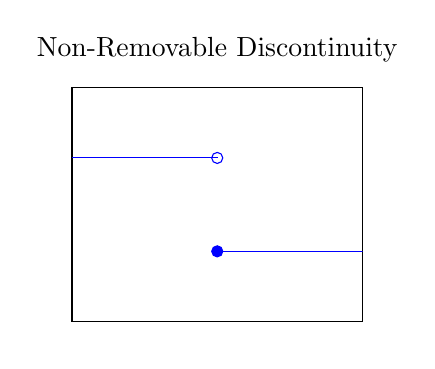
\begin{tikzpicture}
            \begin{axis}[
                    axis lines        = box,
                    xmin              = -5,
                    xmax              = 5,
                    ymin              = -5,
                    ymax              = 5,
                    xtick             = \empty,
                    ytick             = \empty,
                    xlabel            = \empty,
                    ylabel            = \empty,
                    trig format plots = rad,
                    width             = 15em,
                    title             = {Non-Removable Discontinuity}
                ]

                \addplot [
                    smooth,
                    color=blue,
                    domain=-5:0
                ]{2};

                \addplot [
                    smooth,
                    color=blue,
                    domain=0:5
                ]{-2};

                \addplot [
                    color=blue,
                    mark=o
                ]coordinates {(0,2)};

                \addplot [
                    color=blue,
                    mark=*
                ]coordinates {(0,-2)};

            \end{axis}
        \end{tikzpicture}
    }
\end{multicols}

\newpage
\subsubsection{Asymptotes}
\begin{multicols}{2}[
\begin{definition}{Asymptotes}
    \begin{multicols}{2}{
            Vertical asymptote are when:
            \begin{displaymath}
                \lim_{x\to c}f(x)=\pm\infty
            \end{displaymath}
            \\
        }
        {
            Horizontal asymptote is:
            \begin{displaymath}
                \lim_{x\to \pm\infty}f(x)=L
            \end{displaymath}
        }
    \end{multicols}
\end{definition}
]{
\begin{center}
        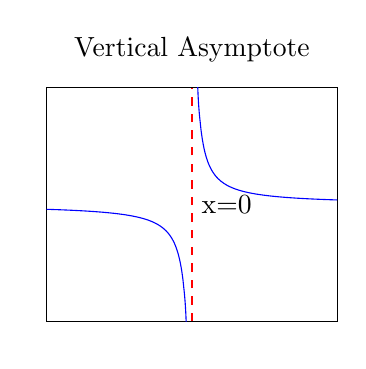
\begin{tikzpicture}
            \begin{axis}[
                    axis lines        = box,
                    xmin              = -5,
                    xmax              = 5,
                    ymin              = -5,
                    ymax              = 5,
                    xtick             = \empty,
                    ytick             = \empty,
                    xlabel            = \empty,
                    ylabel            = \empty,
                    trig format plots = rad,
                    width             = 15em,
                    title             = {Vertical Asymptote}
                ]

                % it draws a vertical line if i don't do this
                \addplot [
                    smooth,
                    color=blue,
                    samples=50,
                    domain=-5:-.1
                ]{1/x};
                \addplot [
                    smooth,
                    color=blue,
                    samples=50,
                    domain=.1:5
                ]{1/x};

                \draw [dashed, red] (0, -5) -- (0, 5);
                \node [right] at (0, 0) {x=0};

            \end{axis}
        \end{tikzpicture}
        $f(x)=\frac{1}{x}$
\end{center}
}
{
\begin{center}
        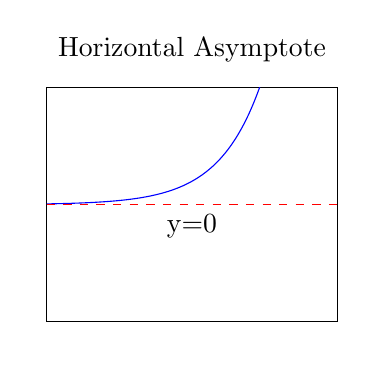
\begin{tikzpicture}
            \begin{axis}[
                    axis lines        = box,
                    xmin              = -5,
                    xmax              = 5,
                    ymin              = -5,
                    ymax              = 5,
                    xtick             = \empty,
                    ytick             = \empty,
                    xlabel            = \empty,
                    ylabel            = \empty,
                    trig format plots = rad,
                    width             = 15em,
                    title             = {Horizontal Asymptote}
                ]

                % it draws a vertical line if i don't do this
                \addplot [
                    smooth,
                    color=blue,
                    samples=50,
                ]{2^x};

                \draw [dashed, red] (-5, 0) -- (5, 0);
                \node [below] at (0, 0) {y=0};

            \end{axis}
        \end{tikzpicture}
        $f(x)=2^x$
\end{center}
}
\end{multicols}

\begin{note}{}
    We can infer something from vertical asymptotes from this graph:
    As the denominator becomes closer to zero, and it's a positive number, then
    the $f(x)$ will approach $\infty$. If the denominator approaches zero and
    is negative, then $f(x)$ will approach $-\infty$
\end{note}

\begin{example}{Curveball Asymptote}
    Find the asymptotes:
    \begin{displaymath}
        f(x)=\frac{\sqrt{(x-1)(x-3)}}{(x-2)(x-4)}
    \end{displaymath}
    \br
    You'd \textit{think} that the asymptotes are $x=\{2, 4\}$, but you must
    consider the \textit{domain} at which $f(x)$ exists.
    \\
    Because this is a square root function, $(x-1)(x-3)$ \textit{cannot be a 
    negative number}. Plugging in $x=2$ would result in a negative square root.
\end{example}

\marginpar{Moral of the story: double-check your answers!}
\begin{example}{Curveball Trigonometry}
    Find the asymptotes:
    \begin{displaymath}
        f(x)=\frac{\sin(x)}{x^3-x}
    \end{displaymath}
    \br
    Let's start by factoring out the denominator:
    \begin{displaymath}
        f(x)=\frac{\sin(x)}{x(x-1)(x+1)}
    \end{displaymath}
    You'd \textit{think} that the asymptotes are $x=\{-1, 0, 1\}$. However,
    $\lim_{x\to 0}f(x)=1$ --- $f(x)$ can also be re-written as this:
    $\lim_{x\to 0}[\frac{\sin x}{x}] \cdot \lim_{x\to 0}[\frac{1}{(x-1)^2}]=-1$
\end{example}

\newpage
\section{Differentiation}

\begin{note}{}
    Derivatives are essentially the \textit{slope} of the function at a
    certain point \\
    They also \textit{cannot exist} where the limit doesn't exist at the 
    function
\end{note}

\subsection{Derivatives and Tangent Lines}
%graph some examples of tanget line
Some mathematicians were trying to find out how to draw a line that intersects 
a function at \textit{only one point}:

\begin{center}
        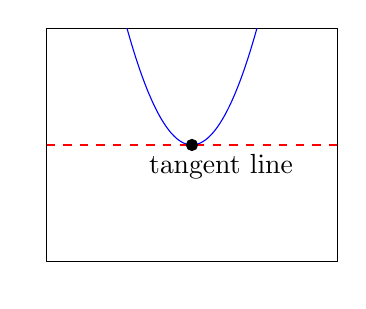
\begin{tikzpicture}
            \begin{axis}[
                    axis lines        = box,
                    xmin              = -5,
                    xmax              = 5,
                    ymin              = -5,
                    ymax              = 5,
                    xtick             = \empty,
                    ytick             = \empty,
                    xlabel            = \empty,
                    ylabel            = \empty,
                    trig format plots = rad,
                    width             = 15em,
                ]

                % it draws a vertical line if i don't do this
                \addplot [
                    smooth,
                    color=blue,
                    samples=50,
                ]{x^2};

                \addplot [
                    color=black,
                    mark=*
                ]coordinates{(0, 0)};

                \draw [dashed, red] (-5, 0) -- (5, 0);

                \node[below] at (1, 0) {tangent line};
            \end{axis}
        \end{tikzpicture}
\end{center}

However, it takes \textit{two points} to draw a line, so they were confuzzled.

You can just Google up the rest of the lore behind the definition of a limit, 
but it boils down to this:
\begin{theorem}{Derivative via. Limits}
    \begin{displaymath}
        \lim_{h\to 0}\frac{f(x+h)-f(x)}{h}=f'(c)\text{ and }
        \lim_{x\to a}\frac{f(x)-f(a)}{x-a}=f'(c)
    \end{displaymath}
\end{theorem}

\begin{note}{Alternative Ways of Writing a Derivative}
There are other ways that mathematicians defined derivative:
\begin{multicols}{2}[]
    \begin{itemize}
        \item $f'(x)$
        \item $\frac{dy}{dx}$
        \item $\frac{d}{dx}f(x)$
        \item $Dx(y)$
    \end{itemize}
\end{multicols}
This isn't essential to know, but it's pretty useful to see how other
mathematicians may express derivatives
\end{note}

\begin{theorem}{Continuity of Derivatives}
    If function $f(x)$ is differentiable at $x=c$, then it is 
    \textit{also continuous} at $x=c$
\end{theorem}

\begin{example}{Finding the Tangent Line}
    Find the tangent lines to $f(x)=x^2+1$ at $(-2, 5)$:
    \br
    Let's start by finding the derivative of the function at $x=-2$:
    \begin{align*}
        f'(-2)&=\lim_{h\to 0}\frac{f(-2+h)-f(-2)}{h} \\
        &=\lim_{h\to 0}\frac{\bigl((-2+h)^2+1\bigr)-(5)}{h} \\
        &=\lim_{h\to 0}\frac{h^2-4h}{h} \\
        &=\lim_{h\to 0}-4+h = -4 + (0)\\
        &=-4\\
    \end{align*}
    Now we must write a point-slope equation with that derivative. 
    \begin{align*}
        y-y_1&=m(x-x_1) \\
        y-(5)&=(-4)(x-(-2)) \\
        y-5&=-4(x+2)
    \end{align*}

    Tangent line to $f(x)=x^2+1$ at $(-2, 5)$ has equation: $$y-5=-4(x+2)$$
\end{example}

Another way to find the derivative of the function would be to find the limit
of $f(x)$ when $x=c$ and then plugging in $c$ with any number that you want:
\begin{align*}
    f'(c)&=\lim_{h\to 0}\frac{f(c+h)-f(c)}{h} \\
    &=\lim_{h\to 0}\frac{\bigl((c+h)^2+1\bigr)-(c^2+1)}{h} \\
    &=\lim_{h\to 0}\frac{(c^2+2ch+h^2+1)-(c^2+1)}{h} \\
    &=\lim_{h\to 0}\frac{2ch+h^2}{h} = \lim_{h\to 0}\frac{h(2c+h)}{h}\\
    &=\lim_{h\to 0} 2c+h=2c+(0)\\
    &=2c\\
    \\
    c&=2\\
    f'(-2)&=2(-2)=-4
\end{align*}

\newpage
\subsection{Rules of Derivatives}
Finding derivatives with the limit definition can get pretty exhausting, so
mathematicians came up with a lot of shortcuts to evaluate derivatives much
quicker. This is a pretty lengthy section, because of the many practice example 
problems I'll be putting in this section, but here are the rules in short:

\begin{align*}
    \text{let: } f(x)&= \text{a function}\\
                 g(x)&= \text{another function}\\
                   c &= \text{a constant}
\end{align*}
\begin{table}[h]
    \label{tab:2.2}
    \begin{center}
        \begin{tabular}{ |c|c| }
            \hline
            Rule & Math Expression\\
            \hline
            \hline
            Constant & $\frac{d}{dx}c=0$\\
            \hline
            Power & $\frac{d}{dx}x^n=nx^{n-1}$\\
            \hline
            Sum and Difference & $\frac{d}{dx}[f(x)\pm g(x)]=f'(x)\pm g'(x)$\\
            \hline
            $\sin$& $\frac{d}{dx}\sin(x)=\cos(x)$\\
            \hline
            $\cos$& $\frac{d}{dx}\cos(x)=-\sin(x)$\\
            \hline
            Product& 
                $\frac{d}{dx}[f(x)g(x)]=f(x)g'(x)+g(x)f'(x)$\\
            \hline
            Quotient& 
                $\frac{d}{dx}[\frac{f(x)}{g(x)}]=
                 \frac{g(x)\cdot f'(x)-f(x)\cdot g'(x)}{\bigl(g(x)\bigr)^2}$\\
            \hline
            Chain & $\frac{d}{dx}f(g(x))=g'(x)\cdot f'(g(x))$\\
            \hline
        \end{tabular}
    \end{center}
\end{table}

\marginpar{You don't have to simplify completely on open-ended questions!}
\begin{example}{Power Rule}
    \begin{multicols}{2}
        \begin{enumerate}
            \item $\frac{d}{dx}(3x^2+4x)=6x+4$
            \item $\frac{d}{dx}\sqrt{x}=\frac{d}{dx}x^{\frac{1}{2}}
                =\frac{1}{2}x^{-\frac{1}{2}}$
            \item $\frac{d}{dx}\sqrt[3]{x^2}=\frac{d}{dx}x^{\frac{2}{3}}
                =x^{-\frac{1}{3}}$
        \end{enumerate}
    \end{multicols}
\end{example}

\begin{example}{$\sin$/$\cos$ Rule}
    \begin{enumerate}
        \item $\frac{d}{dx}
            \bigl(2\sin(\theta)+3\cos(\theta)-\frac{4}{\theta}\bigr)=
            2\cos(\theta)-3\sin(\theta)+\frac{4}{\theta^2}
            $
        \item $\frac{d}{dx}\bigl(x^2+2\cos(x)\bigr)=2x-2\sin(x)$
    \end{enumerate}
\end{example}

\begin{example}{Find Horizontal Tangents}
    Find the horizontal tangents of $f(x)=x^4-2x^2+3$:
    \br
    The question is essentially asking us when the slope of the functions are
    equal to 0
\end{example}

\newpage
\section{Cheat Sheet}
\begin{multicols}{2}
    \begin{GrayBox}{Limits}{}
        $\lim_{x\to c}f(x)=L$
    \end{GrayBox}
\end{multicols}
\end{document}
